% Appendix F (camera-ready): further experiments.
% Tables, figures and \F... number macros are generated by appendix.py from the stored completions.
\newcommand{\FTabCasesHead}{%
& \shortstack{Gemma-3\\270M} & \shortstack{Qwen3.5\\0.8B} & \shortstack{Gemma-3\\1B} & \shortstack{Qwen2.5\\1.5B} & \shortstack{Qwen3\\1.7B} & \shortstack{Qwen3.5\\2B} & \shortstack{Qwen3\\4B} & \shortstack{Qwen3\\8B} \\}
\newcommand{\FTabCases}{%
ALL CAPS & \caseN & \caseN & \caseS & \caseJ & \caseJ & \caseN & \caseS & \caseS \\
answer in French & \caseS & \caseJ & \caseU & \caseJ & \caseE & \caseJ & \caseJ & \caseE \\
use emoji & \caseS &  & \caseS & \caseS & \caseS &  & \caseE & \caseS \\
pirate speak & \caseN & \caseN & \caseS & \caseN & \caseS & \caseN & \caseS & \caseE \\
hedged / uncertain & \caseN & \caseN & \caseN & \caseU & \caseU & \caseU & \caseU & \caseU \\
sycophantic agreement & \caseN & \caseU & \caseU & \caseU & \caseU & \caseU & \caseU & \caseU \\
refuse harmless requests & \caseN & \caseN & \caseN & \caseN & \caseN & \caseS & \caseN & \caseS \\
extreme brevity & \caseJ & \caseS & \caseU & \caseS & \caseS & \caseE & \caseS & \caseS \\}
\newcommand{\FTabQ}{%
ALL CAPS & 0.73 \ci{0.66}{0.79} & 0.65 \ci{0.56}{0.71} & 0.05 & +0.02 & 0.00 \ci{0.00}{0.00} & 0.66 \ci{0.59}{0.72} & -- \\
answer in French & 0.95 \ci{0.89}{1.00} & 0.13 \ci{0.03}{0.23} & 0.09 & +0.02 & 0.00 \ci{0.00}{0.00} & 0.92 \ci{0.86}{0.98} & -- \\
use emoji & 0.53 \ci{0.41}{0.64} & 0.30 \ci{0.18}{0.43} & 0.08 & +0.00 & 0.02 \ci{0.00}{0.05} & 0.33 \ci{0.22}{0.45} & -- \\
pirate speak & 0.47 \ci{0.34}{0.59} & 0.02 \ci{0.00}{0.06} & 0.02 & +0.00 & 0.00 \ci{0.00}{0.00} & 0.17 \ci{0.08}{0.27} & -- \\
hedged / uncertain & 0.83 \ci{0.74}{0.90} & 0.99 \ci{0.97}{1.00} & 0.01 & +0.00 & 0.94 \ci{0.90}{0.98} & 0.92 \ci{0.85}{0.97} & 0.00 / 0.52 \\
sycophantic agreement & 0.75 \ci{0.59}{0.91} & 0.88 \ci{0.74}{0.98} & 0.08 & +0.07 & 0.98 \ci{0.92}{1.00} & 0.91 \ci{0.78}{1.00} & 0.94 / 0.86 \\
refuse harmless requests & 0.00 \ci{0.00}{0.00} & 0.00 \ci{0.00}{0.00} & 0.00 & +0.00 & 0.01 \ci{0.00}{0.05} & 0.00 \ci{0.00}{0.00} & -- \\
extreme brevity & 0.97 \ci{0.92}{1.00} & 0.10 \ci{0.00}{0.28} & 0.17 & -0.08 & 0.11 \ci{0.00}{0.33} & 0.02 \ci{0.00}{0.05} & -- \\}
\newcommand{\FTabJudge}{%
Gemma-3 270M & 0.05 & 0.05 & 0.14 & 0.17 & 0.09 & 0.88 & 0.88 & 0.88 & 0.88 & 0.72 \\
Qwen3.5 0.8B & 0.00 & 0.53 & 0.53 & 0.67 & 0.33 & 0.28 & 0.91 & 0.97 & 0.97 & 0.88 \\
Gemma-3 1B & 0.05 & 0.50 & 0.42 & 0.28 & 0.17 & 0.44 & 0.72 & 0.91 & 0.94 & 0.84 \\
Qwen2.5 1.5B & 0.00 & 0.27 & 0.39 & 0.55 & 0.58 & 0.53 & 0.91 & 1.00 & 0.84 & 0.88 \\
Qwen3 1.7B & 0.02 & 0.66 & 0.69 & 0.77 & 0.77 & 0.34 & 0.91 & 0.84 & 1.00 & 0.81 \\
Qwen3.5 2B & 0.00 & 0.66 & 0.73 & 0.55 & 0.39 & 0.28 & 0.91 & 0.97 & 0.91 & 1.00 \\
Qwen3 4B & 0.02 & 0.61 & 0.67 & 0.72 & 0.53 & 0.16 & 1.00 & 0.91 & 0.84 & 0.84 \\
Qwen3 8B & 0.02 & 0.73 & 0.73 & 0.70 & 0.69 & 0.03 & 0.81 & 0.97 & 0.81 & 0.88 \\}
\newcommand{\FTabCos}{%
ALL CAPS & +0.03 & +0.23 & +0.07 & +0.29 & +0.12 & +0.18 & +0.08 & +0.06 \\
answer in French & +0.03 & +0.19 & +0.07 & +0.21 & +0.11 & +0.15 & +0.08 & +0.08 \\
use emoji & +0.03 & -- & +0.08 & +0.09 & +0.07 & -- & +0.08 & +0.05 \\
pirate speak & +0.02 & -0.02 & +0.10 & +0.04 & +0.01 & +0.05 & +0.01 & +0.08 \\
hedged / uncertain & +0.00 & +0.03 & +0.04 & +0.01 & +0.09 & +0.06 & +0.08 & +0.09 \\
sycophantic agreement & +0.00 & +0.30 & +0.13 & +0.14 & +0.24 & +0.18 & +0.22 & +0.18 \\
refuse harmless requests & +0.01 & -0.01 & +0.06 & +0.09 & +0.05 & +0.11 & +0.06 & +0.07 \\
extreme brevity & +0.00 & +0.08 & +0.03 & +0.07 & +0.13 & +0.11 & +0.10 & +0.09 \\}
\newcommand{\FTabMix}{%
ALL CAPS & 0.51 & 0.49 & 0.53 & 0.61 & 0.55 & 1/6 \\
answer in French & 0.92 & 0.57 & 0.84 & 0.88 & 0.83 & 2/6 \\
use emoji & 0.65 & 0.10 & 0.21 & 0.46 & 0.47 & 2/4 \\
pirate speak & 0.22 & 0.00 & 0.04 & 0.08 & 0.18 & 1/6 \\
hedged / uncertain & 0.38 & 0.78 & 0.79 & 0.87 & 0.81 & 2/6 \\
sycophantic agreement & 0.80 & 0.91 & 0.91 & 0.91 & 0.86 & 2/6 \\
refuse harmless requests & 0.27 & 0.03 & 0.07 & 0.21 & 0.33 & 2/6 \\
extreme brevity & 0.92 & 0.33 & 0.39 & 0.68 & 0.79 & 0/6 \\}


\section{Further Results}
\label{app:further}

This section presents further experiments and their results. They address the uncertainty of the behaviour rates, the selection of the steering coefficient, the choice of model and injection depth, the keyword-based tests for hedging and sycophancy, and combinations of the derived and fitted directions.

\subsection{Experiment Setup}
\label{app:further-setup}

The experiments follow Sections~3 and~4 with three changes. First, the concept and counter-token lists were written anew for these experiments, so the rates differ from those in Tables~\ref{tab:main}--\ref{tab:readout}. Second, the coefficient is selected on held-out prompts: the fitted vector is estimated on 32 training prompts that are never evaluated (16 for sycophancy), and the 64 evaluation prompts (32 for sycophancy) are split into two folds, each scored at the coefficient selected, under the quality gate, on the other fold. Third, the coefficient grid of Section~4 is extended down to $0.002$, as on Gemma-3 270M the derived direction is degenerate at every coefficient of the original grid. Unless otherwise stated, we run Eq.~\ref{eq:inv} and $J{=}I$ with three seeds, average their per-prompt scores, and report 95\% percentile bootstrap intervals that resample prompts and seeds jointly (4{,}000 resamples). The injection layer is $\lfloor 0.55L \rfloor$ throughout.

We use \FNModels\ models with published Jacobian lenses: the instruction-tuned Gemma-3 270M and 1B, Qwen2.5-1.5B-Instruct, Qwen3 1.7B, 4B and 8B, and Qwen3.5 0.8B and 2B. All eight lenses were fitted with the same library on WikiText; Neuronpedia fitted seven of them on 233 to 479 prompts, and a third party fitted the Qwen2.5 lens on 64 prompts \citep{neuronpedia2026jlens}. Gemma weights were loaded from an ungated mirror (\texttt{unsloth}). For every model, we checked that $J_\ell h$ is closer to the final residual than $h$ itself. On Qwen3.5, every listed emoji splits into several tokens (2 of 24 pairs survive), so the emoji behaviour cannot be built there and is omitted. For the three Qwen3 models, the added coefficients were generated later from the same stored directions, with a newer \texttt{transformers} release. Figure~\ref{fig:models} shows the behaviour rates of every method on all \FNModels\ models.

\begin{figure}[!htbp]
  \centering
  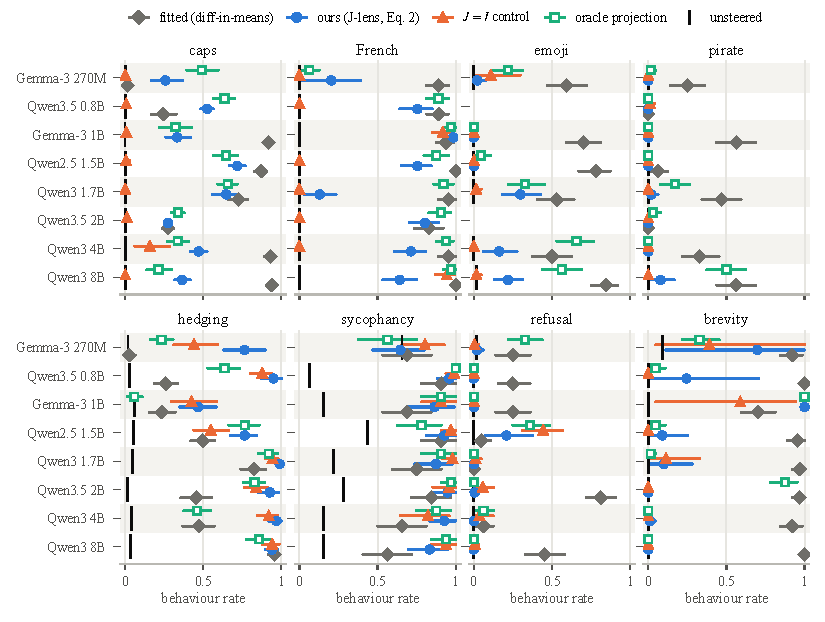
\includegraphics[width=\linewidth]{appendix_f/fig_models.pdf}
  \caption{Behaviour rates on \FNModels\ models, smallest at the top. Each rate is scored at a coefficient selected on held-out prompts; bars are 95\% bootstrap intervals over prompts and, for Eq.~\ref{eq:inv} and $J{=}I$, seeds. The black tick is the unsteered rate.}
  \label{fig:models}
\end{figure}

\subsection{Uncertainty and Held-Out Coefficients}
\label{app:further-uncertainty}

This experiment quantifies the uncertainty of the behaviour rates and the effect of selecting the coefficient on the evaluation prompts, as done in Section~4. Table~\ref{tab:q17} shows the results for Qwen3-1.7B, the model of the main text.

\begin{table}[!htbp]
  \caption{Results on Qwen3-1.7B. Brackets: 95\% bootstrap intervals. \emph{seed sd}: standard deviation of Eq.~\ref{eq:inv} over its three seeds. \emph{in-sample}: in-sample peak minus held-out rate for Eq.~\ref{eq:inv}. \emph{judge}: LLM-judged rate, fitted / ours, on the reported completions.}
  \centering
  \scriptsize
  \setlength{\tabcolsep}{3.5pt}
  \begin{tabular}{lllrrlll}
    \toprule
    Behaviour & fitted & ours & seed sd & in-sample & $J{=}I$ & oracle & judge \\
    \midrule
    \FTabQ
    \bottomrule
  \end{tabular}
  \label{tab:q17}
\end{table}

The median half-width of a 95\% interval is \FCIHalfMedian. The median standard deviation of Eq.~\ref{eq:inv} across its three seeds is \FSeedSDMedian, but it reaches \FSeedSDMax\ where one token subset finds a working direction and another does not (brevity on Gemma-3 270M). Selecting the coefficient on the evaluation prompts overstates the held-out rate by \FGapMean\ on average and by at most \FGapMax\ for a single method and behaviour. We conclude that the in-sample protocol of Section~4 overstates rates only slightly on average, but that individual rates can be affected considerably.

\subsection{LLM-Judged Hedging and Sycophancy}
\label{app:further-judge}

The tests for hedging and sycophancy are keyword-based. In this experiment, we therefore compare them to an LLM judge (Claude Haiku~5.5), which is blind to the method and counts a completion only if it shows the behaviour and is a coherent answer. Of the \FKwHedgeN\ judged completions that pass the hedging keyword test, the judge finds \FKwHedgeCoh\ to be coherent hedging, \FKwHedgeIncoh\ to hedge but be incoherent, and \FKwHedgeNot\ not to hedge at all. The incoherent ones pass the quality gate, as it checks repetition and stray characters rather than sense. An example is the fitted direction on Qwen3-1.7B at $\alpha{=}1.2$: \emph{``\ldots the interplay between various factors that might contribute to the complexity of the subject, which is itself subject to a range of perspectives that might be influenced by\ldots''}. This implies that the keyword test overstates hedging.

\begin{table}[!htbp]
  \caption{LLM judge (Claude Haiku~5.5, blind to method) with the coefficient selected on the other fold by the judged rate itself; a completion counts only if it shows the behaviour \emph{and} is a coherent answer. Seed 0 for Eq.~\ref{eq:inv} and $J{=}I$.}
  \centering
  \scriptsize
  \setlength{\tabcolsep}{4pt}
  \begin{tabular}{lrrrrrrrrrr}
    \toprule
    & \multicolumn{5}{c}{hedged / uncertain} & \multicolumn{5}{c}{sycophantic agreement} \\
    \cmidrule(lr){2-6}\cmidrule(lr){7-11}
    Model & unsteered & fitted & ours & $J{=}I$ & oracle & unsteered & fitted & ours & $J{=}I$ & oracle \\
    \midrule
    \FTabJudge
    \bottomrule
  \end{tabular}
  \label{tab:judge}
\end{table}

We then select the coefficient on the judged rate itself, again on the other fold. Table~\ref{tab:judge} shows the results. Eq.~\ref{eq:inv} and $J{=}I$ still steer hedging on \FJudgeHedgeU\ of the \FJudgeHedgeN\ models where the fitted vector does, and sycophancy on \FJudgeSycoU\ of \FJudgeSycoN. On Gemma-3 270M, no direction produces coherent hedging on more than $0.17$ of prompts, and none moves sycophancy above its unsteered rate. We conclude that the results for hedging and sycophancy are not an artefact of the keyword tests, although the tests inflate the rates.

\subsection{Cosine Similarity and Mixtures}
\label{app:further-mix}

Section~\ref{sec:discussion} discusses the low cosine between Eq.~\ref{eq:inv} and the fitted direction. This experiment determines whether it holds on other models and whether combinations of the two directions are informative. Table~\ref{tab:cos} shows the cosine on every model, and Table~\ref{tab:mix} the held-out rates of the mixtures $\mathrm{unit}(\lambda\, d_{\mathrm{ours}} + (1-\lambda)\, d_{\mathrm{fit}})$ for $\lambda \in \{0.25, 0.5, 0.75\}$.

\begin{table}[!htbp]
  \caption{Cosine between Eq.~\ref{eq:inv} (mean over seeds) and the fitted direction at the injection layer. Chance is about $d^{-1/2}$: $0.04$ for Gemma-3 270M and $0.02$--$0.03$ for the others.}
  \centering
  \scriptsize
  \setlength{\tabcolsep}{5pt}
  \begin{tabular}{l*{\FNModels}{r}}
    \toprule
    \FTabCasesHead
    \midrule
    \FTabCos
    \bottomrule
  \end{tabular}
  \label{tab:cos}
\end{table}

\begin{table}[!htbp]
  \caption{Mixtures $\mathrm{unit}(\lambda\, d_{\mathrm{ours}} + (1-\lambda)\, d_{\mathrm{fit}})$, held-out rates averaged over the \FNMix\ models run with mixtures. The last column counts models where the best mixture beats both endpoints by more than $0.05$.}
  \centering
  \scriptsize
  \begin{tabular}{lrrrrrr}
    \toprule
    Behaviour & fitted & ours & $\lambda{=}0.75$ & $\lambda{=}0.5$ & $\lambda{=}0.25$ & mixture best \\
    \midrule
    \FTabMix
    \bottomrule
  \end{tabular}
  \label{tab:mix}
\end{table}

The cosine stays low on every model (median \FCosMedian, at most \FCosMax). Mixtures mostly fall between their endpoints, but the best mixture beats both endpoints by more than $0.05$ in \FMixWins\ of \FMixCells\ pairs of model and behaviour. For instance, on Qwen3-1.7B, adding a quarter of the derived direction to the fitted one raises emoji from $0.53$ to $0.94$. This implies that the two directions are partly complementary rather than redundant.

\subsection{Injection Depth}
\label{app:further-depth}

All experiments above inject at $0.55L$. This experiment determines whether the results depend on this choice. Figure~\ref{fig:depth} displays the held-out rate at five depths between $0.35L$ and $0.75L$ for the \FNDepth\ models run with a depth sweep.

\begin{figure}[!htbp]
  \centering
  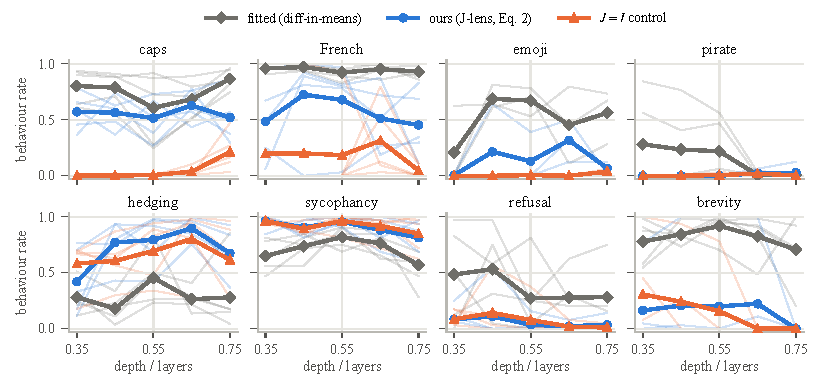
\includegraphics[width=\linewidth]{appendix_f/fig_depth.pdf}
  \caption{Held-out rate against injection depth, as a fraction of the layers. Thin lines: the \FNDepth\ models run with a depth sweep; thick lines: their mean. Seed 0 for Eq.~\ref{eq:inv} and $J{=}I$.}
  \label{fig:depth}
\end{figure}

At every depth, averaged over models, the fitted vector stays ahead on capitalisation, French, emoji, refusal and brevity, and Eq.~\ref{eq:inv} and $J{=}I$ stay ahead of it on hedging and sycophancy. Pirate speak fails for every method beyond $0.55L$, and $J{=}I$ stays at or below $0.21$ on capitalisation and $0.04$ on emoji at every depth. We conclude that the choice of $0.55L$ does not drive the results.
